\documentclass[runningheads]{llncs}
\usepackage[UTF8]{ctex}
\usepackage{amsmath,amssymb}
\usepackage{graphicx}
\usepackage{booktabs}
\usepackage{multirow}
\usepackage{url}
\usepackage{hyperref}
\usepackage{xcolor}
\usepackage{enumitem}

\newcommand{\todo}[1]{\textcolor{red}{\textbf{[TODO: #1]}}}

\begin{document}

\title{IntentAgent：面向检索增强生成的\\意图感知渐进式智能检索方法}

\author{Author Names}
\institute{Institute Names}

\maketitle

\begin{abstract}
检索增强生成（Retrieval-Augmented Generation, RAG）系统的性能高度依赖于检索阶段的质量，然而现有方法普遍采用统一的检索策略处理所有查询，忽视了用户查询意图的多样性对检索路径选择的决定性影响。本文提出IntentAgent，一种面向RAG的意图感知渐进式智能检索方法，其核心思想是：不同意图类型的查询应当被路由到差异化的检索策略，且这一路由过程应从静态规则逐步演化为动态自适应决策。IntentAgent包含三个递进阶段：（1）基于大语言模型与规则双路分类器的六类意图识别及静态策略路由；（2）基于有向状态图的动态工具编排，以推理-行动协议驱动大语言模型自主选择检索工具并引入反思回路实现质量闭环；（3）经验记忆增强机制，通过意图分桶的持久化经验存储实现"入口读—核心用—出口写"三段式闭环，使系统具备跨会话的自我进化能力。在HotpotQA、2WikiMultiHopQA和MuSiQue三个多跳问答基准上的实验表明，IntentAgent在多个骨干模型（Qwen3-8B、Qwen3-32B）下均取得了优于现有文本检索、图检索和混合检索方法的性能。

\textbf{关键词}：检索增强生成；意图分类；动态检索策略；经验记忆；智能体；多跳问答
\end{abstract}
 、
\section{引言}

检索增强生成（Retrieval-Augmented Generation, RAG）通过在大语言模型（Large Language Model, LLM）的生成过程中引入外部知识检索，已成为缓解模型幻觉、提升回答事实性的主流范式~\cite{ref1}。典型的RAG系统遵循"检索—阅读—生成"的三阶段流水线：给定用户查询，先从知识库中检索相关文档片段，再将其作为上下文注入LLM以生成最终回答~\cite{ref2}。

然而，现有RAG系统在检索阶段普遍存在一项隐含的假设局限——\textbf{策略同质性假设}：无论用户查询的意图类型如何，系统均采用相同的检索管道（通常为单次向量相似度检索）。当面对真实场景中的多样化查询时，这一假设的局限性十分突出。考察以下三类查询：

\begin{itemize}[leftmargin=*]
    \item \textbf{事实型查询}（"谁发明了万维网？"）：仅需单次向量检索即可命中答案所在片段；
    \item \textbf{多跳推理查询}（"爱因斯坦的母校对量子力学的发展有何影响？"）：需要跨越多个实体进行桥接推理，单次检索往往无法覆盖完整证据链；
    \item \textbf{对比型查询}（"比较BERT和GPT在文本分类任务上的表现"）：需要并行检索两个实体的相关信息并进行结构化对比。
\end{itemize}

上述三类查询所需的最优检索路径存在显著差异。若将多跳推理查询直接套用单次向量检索管道，往往导致证据不完整甚至缺失；反之，对简单事实型查询使用复杂的多跳检索策略，则会引入不必要的延迟和计算开销。

\begin{figure*}[htbp]
\centering
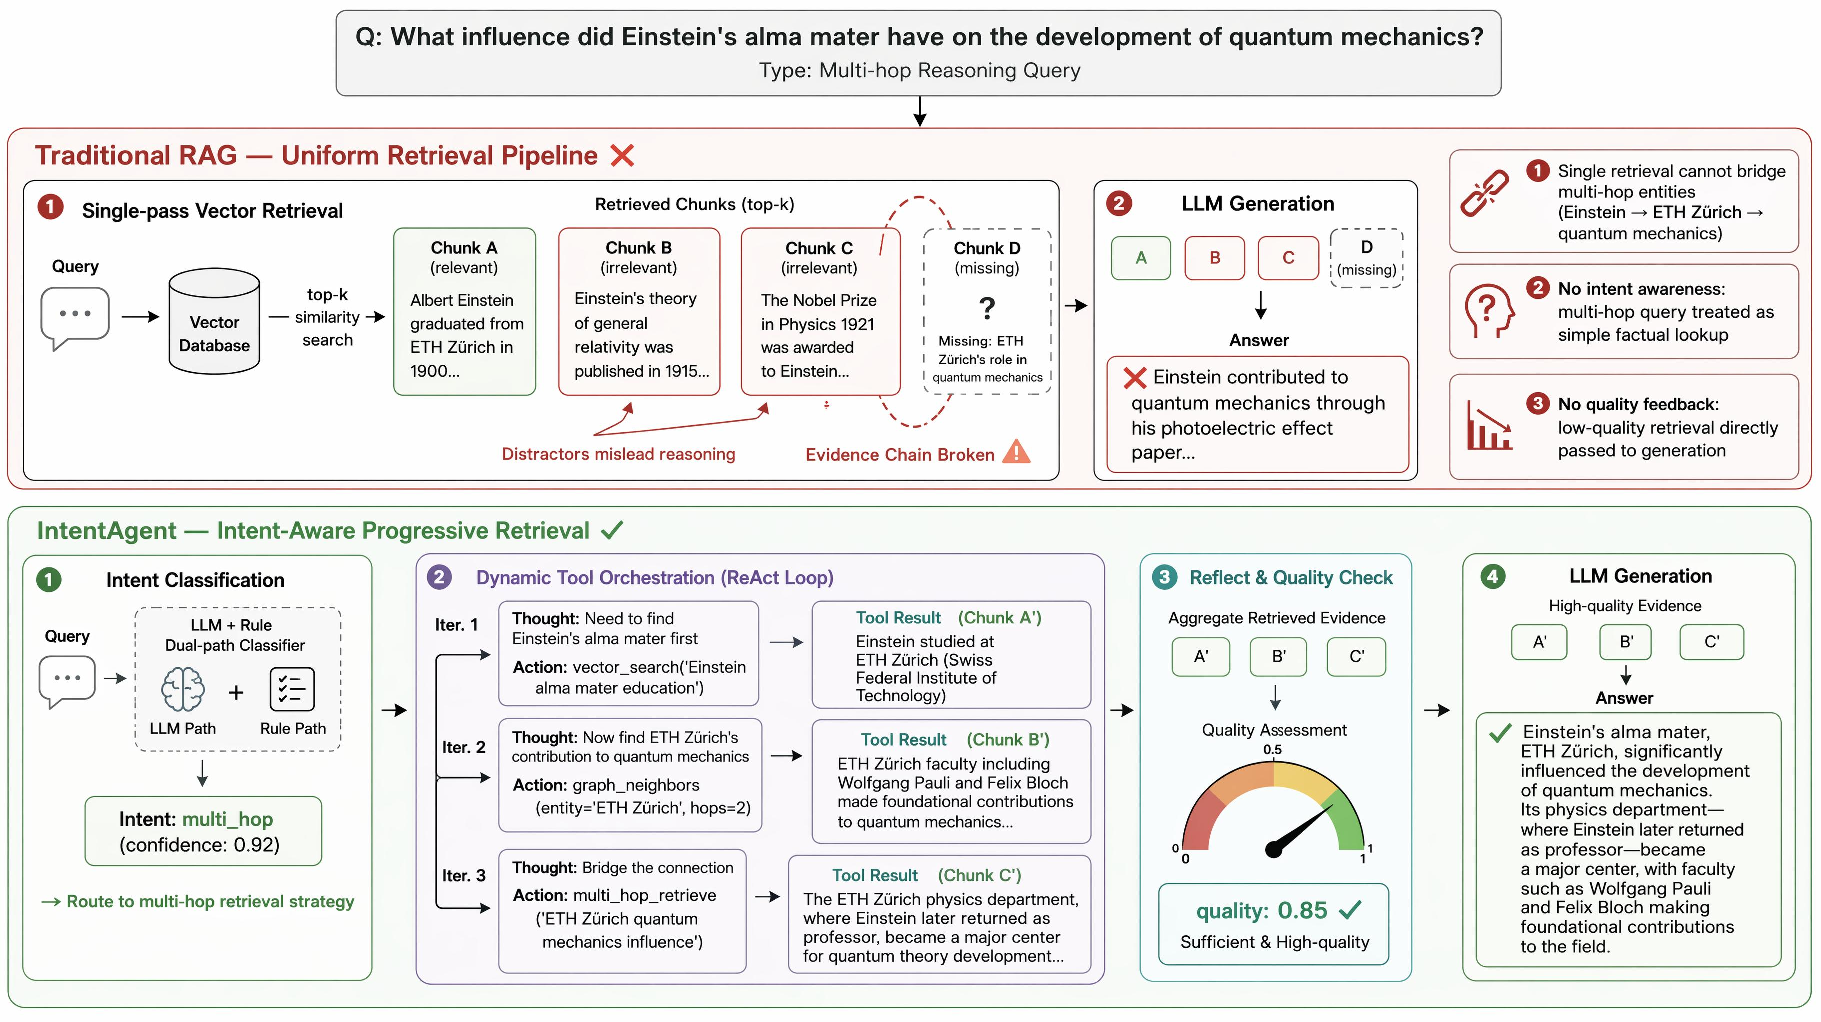
\includegraphics[width=\textwidth]{figures/figure1.pdf}
\caption{传统RAG与IntentAgent的处理流程对比。以多跳推理查询"爱因斯坦的母校对量子力学的发展有何影响？"为例，上半部分展示传统RAG因策略同质性导致的证据链断裂和干扰项误导，下半部分展示IntentAgent通过意图感知的渐进式检索成功收集完整证据链并生成高质量回答。}
\label{fig:comparison}
\end{figure*}

本文提出的核心命题是：\textbf{查询意图应当成为检索策略选择的一等公民}（Query intent should be a first-class citizen in retrieval strategy selection）。我们将这一命题具体化为IntentAgent方法，其设计思路是通过\textbf{三阶段渐进演化}在可控性与自适应性之间取得平衡：

\textbf{阶段一：静态意图路由}。我们首先定义一个涵盖六类查询意图的分类体系（factual, analytical, comparative, multi\_hop, exploratory, follow\_up），并设计LLM与规则级联的双路分类器。分类结果通过确定性映射表路由到预定义的检索策略。

\textbf{阶段二：动态工具编排}。静态路由的局限在于无法处理跨意图查询和运行时自适应。我们引入有向状态图将检索过程重构为LLM驱动的工具选择循环：LLM基于推理-行动协议~\cite{ref13}自主决定调用哪些检索工具、以何种顺序组合，并通过反思节点对已收集证据进行质量评估，在质量不达标时触发重新规划。

\textbf{阶段三：经验记忆增强}。动态编排的每次决策都从零开始，无法利用历史经验。我们设计了基于意图分桶的持久化经验存储，实现"入口读—核心用—出口写"的三段式闭环，使系统具备跨会话的自我进化能力。

我们在HotpotQA~\cite{ref20}、2WikiMultiHopQA~\cite{ref21}和MuSiQue~\cite{ref22}三个多跳问答基准上进行了系统实验，在Qwen3-8B和Qwen3-32B两个骨干模型下评测IntentAgent的效果。实验结果表明，IntentAgent在所有数据集和骨干模型上均取得了优于现有代表性方法（包括Vanilla RAG、RAPTOR~\cite{ref23}、TOG~\cite{ref24}、G-Retriever~\cite{ref25}、LightRAG~\cite{ref26}、GraphRAG~\cite{ref27}和HippoRAG~\cite{ref28}）的性能。

本文的主要贡献如下：
\begin{enumerate}[leftmargin=*]
    \item \textbf{意图感知检索范式}：系统化地将查询意图建模为检索策略选择的主要依据，定义了覆盖主要查询类型的六类意图分类体系及对应的差异化检索策略族，将检索过程从统一匹配转变为意图驱动的差异化检索。
    \item \textbf{三阶段渐进演化方法}：提出从静态路由到动态编排再到经验记忆的渐进式设计，每一阶段针对上一阶段的局限进行改进，在可控性与自适应性之间逐步推进。
    \item \textbf{反思式智能体工具编排}：将检索过程建模为LLM驱动的有向状态图，通过决策—工具调用—反思的回路实现质量门控的自适应检索，使智能体在多种检索原语间自主组合。
    \item \textbf{经验记忆增强机制}：通过意图分桶的持久化经验存储和三段式闭环，赋予RAG系统跨会话的自我进化能力，使同类查询的检索效果随使用次数增加而持续改善。
\end{enumerate}

\section{相关工作}

\subsection{检索增强生成}

检索增强生成（RAG）最早由Lewis等人~\cite{ref1}提出，将信息检索与序列到序列生成相结合，通过在推理时动态检索外部知识来增强语言模型的输出质量。随后，Borgeaud等人~\cite{ref3}提出的RETRO将检索机制深度集成到Transformer架构中。Gao等人~\cite{ref2}对RAG技术栈进行了系统综述，将其划分为朴素RAG、高级RAG和模块化RAG三个演进阶段。

在检索策略层面，\textbf{查询改写路线}通过重写用户查询来提升检索质量，代表工作包括HyDE~\cite{ref4}和Query2Doc~\cite{ref5}。\textbf{多步检索路线}通过迭代式检索逐步收集证据，代表工作包括Self-RAG~\cite{ref6}和CRAG~\cite{ref7}。

在图增强检索方面，GraphRAG~\cite{ref27}利用社区结构对知识图谱进行层次化摘要。LightRAG~\cite{ref26}通过双层检索实现轻量级的图增强检索。HippoRAG~\cite{ref28}借鉴人脑海马体的记忆机制。TOG~\cite{ref24}将LLM作为智能体在知识图谱上进行推理导航。G-Retriever~\cite{ref25}通过图神经网络实现联合检索。RAPTOR~\cite{ref23}通过递归聚类和摘要构建层次化检索树。

然而，上述工作均未将查询意图作为检索策略选择的显式依据。本文的IntentAgent与这些工作的主要区别在于：\textbf{在检索发生之前}，主动识别查询意图并据此选择最适配的检索路径。

\subsection{意图识别与查询理解}

查询意图识别在信息检索和对话系统领域有着悠久的研究历史。Broder~\cite{ref8}最早将Web搜索意图划分为导航型、信息型和事务型三类。后续工作在此基础上不断细化~\cite{ref9,ref10}。在对话系统领域，意图识别通常作为自然语言理解模块的核心任务~\cite{ref11}。近年来，LLM的零样本/少样本分类能力为意图识别提供了新的技术路线~\cite{ref12}。

本文的意图分类体系与上述工作的关键区别在于：我们的六类意图分类是\textbf{面向检索策略差异化}而非面向用户目标理解而设计的。每一类意图直接对应一种检索策略的最优适用场景。

\subsection{基于智能体的检索与经验学习}

ReAct~\cite{ref13}提出了推理与行动交织的范式。Tree of Thoughts~\cite{ref14}将搜索过程建模为树状探索。Toolformer~\cite{ref15}展示了LLM自主学习调用API的能力。

在经验学习方面，Reflexion~\cite{ref16}提出了基于语言反馈的强化学习范式。Voyager~\cite{ref17}实现了技能库的自动积累与复用。MemoRAG~\cite{ref18}探索了将检索经验纳入长期记忆的可能性。

本文的工作在以下方面推进了上述研究：（1）将意图分类作为智能体的先验信息注入；（2）设计了显式的反思回路实现质量门控；（3）通过意图分桶的经验存储机制赋予智能体跨会话的学习能力。

\section{方法}

本节详述IntentAgent的技术方案。我们首先给出问题形式化定义（\S3.1），随后介绍系统总览（\S3.2），之后分三个小节分别阐述三个渐进阶段：静态意图路由（\S3.3）、动态工具编排（\S3.4）和经验记忆增强（\S3.5）。

\subsection{问题形式化}

给定一个知识库$\mathcal{K} = \{d_1, d_2, \ldots, d_N\}$（由$N$篇文档经分块后产生的文本片段集合）以及基于$\mathcal{K}$构建的知识图谱$\mathcal{G} = (\mathcal{V}, \mathcal{E})$（其中$\mathcal{V}$为实体集合，$\mathcal{E}$为关系三元组集合），用户提交查询$q$，RAG系统的目标是检索一个证据集合$\mathcal{R}(q) \subseteq \mathcal{K}$，并基于$\mathcal{R}(q)$生成回答$a$。

传统RAG系统使用固定的检索函数$f_{\text{retrieve}}: q \mapsto \mathcal{R}(q)$，对所有查询施加相同的检索逻辑。我们的核心主张是：最优检索函数应当依赖于查询的意图类型。形式化地，我们定义意图分类函数$\phi: q \mapsto l \in \mathcal{L}$，其中$\mathcal{L} = \{\texttt{factual}, \texttt{analytical}, \texttt{comparative}, \texttt{multi\_hop}, \texttt{exploratory}, \texttt{follow\_up}\}$为六类意图标签集合；以及策略族$\mathcal{S} = \{s_l\}_{l \in \mathcal{L}}$，其中每个策略$s_l$是面向意图$l$优化的检索函数。IntentAgent的目标函数可以表述为：
\begin{equation}
    \mathcal{R}^*(q) = s_{\phi(q)}(q, \mathcal{K}, \mathcal{G})
\end{equation}
即先识别查询意图，再将查询路由到对应的最优策略执行检索。三阶段渐进演化体现在策略选择机制$s_{\phi(q)}$的逐步智能化：从确定性映射（阶段一）到LLM驱动的动态选择（阶段二）再到经验增强的自适应决策（阶段三）。

\subsection{系统总览}

\begin{figure*}[htbp]
\centering
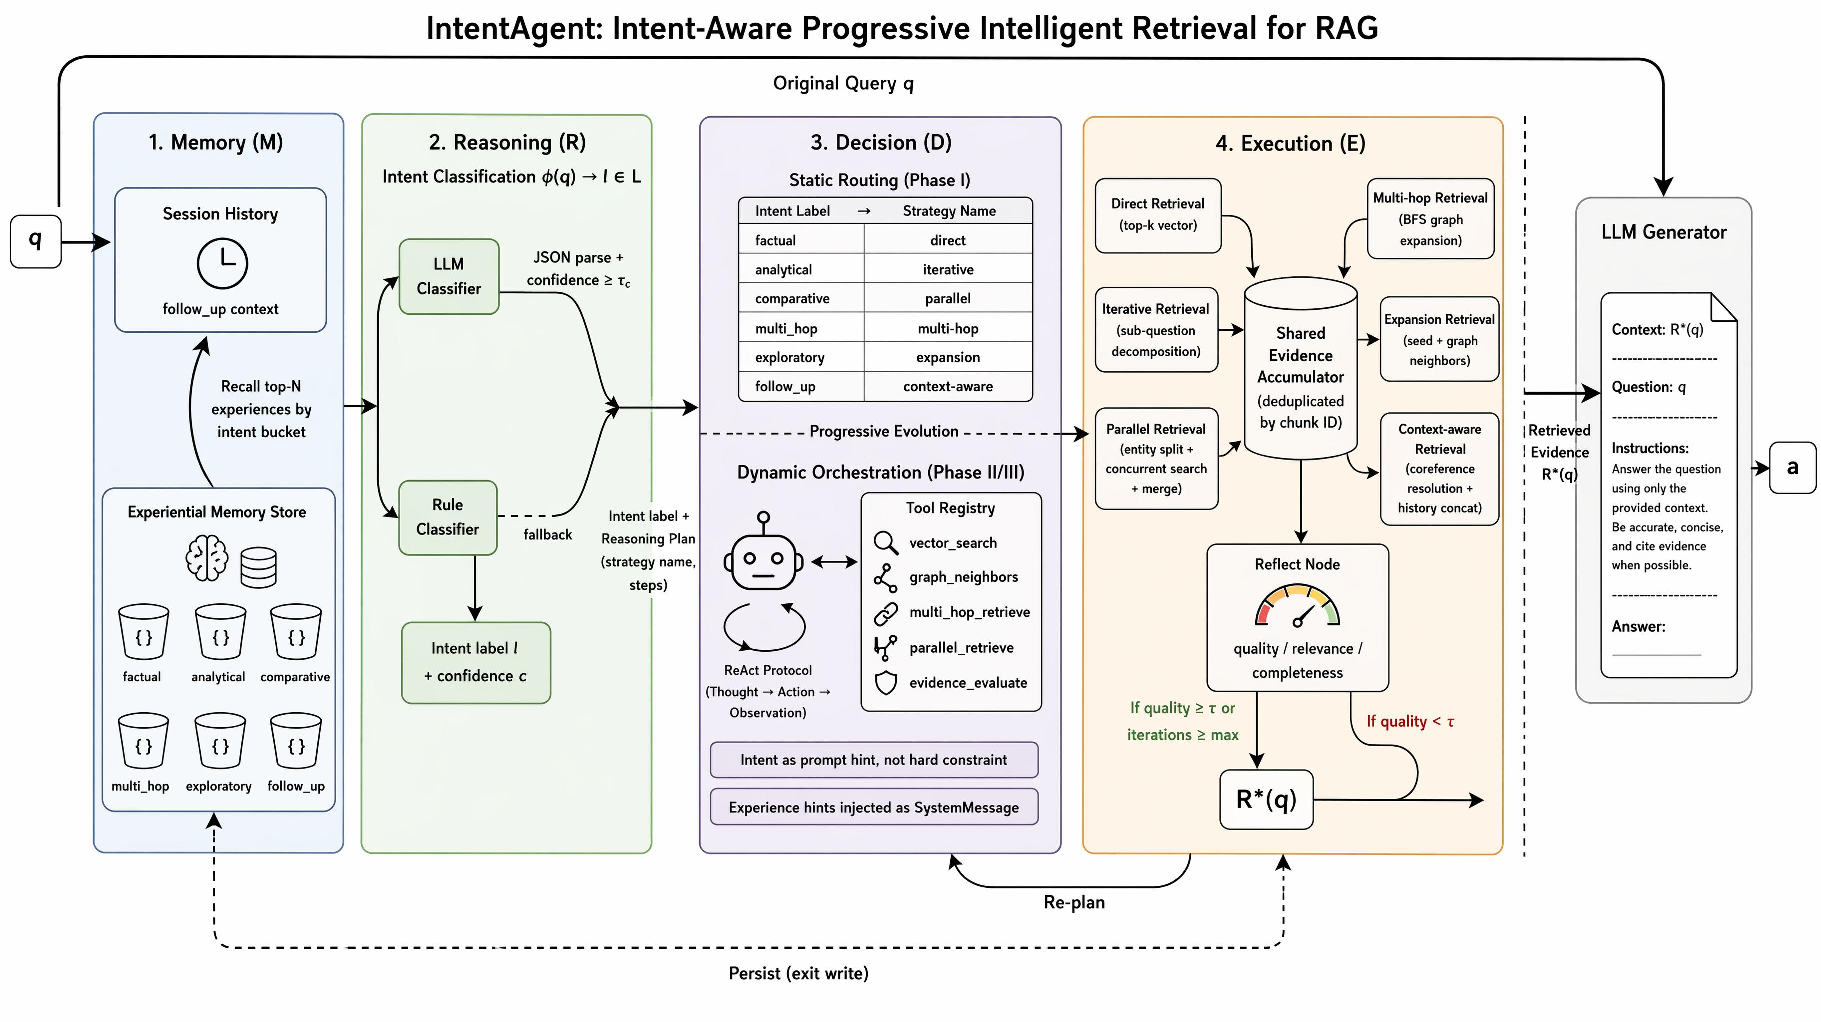
\includegraphics[width=\textwidth]{figures/figure2.pdf}
\caption{IntentAgent总体架构图。系统遵循M-R-D-E四阶段处理流水线：Memory阶段读取会话历史与经验记忆，Reasoning阶段通过LLM+规则双路分类器识别六类查询意图，Decision阶段在静态映射（阶段一）或状态图动态编排（阶段二/三）间切换，Execution阶段执行差异化检索策略并通过反思节点进行质量门控。三个渐进演化阶段的覆盖范围以不同颜色标注。}
\label{fig:architecture}
\end{figure*}

IntentAgent遵循Memory $\to$ Reasoning $\to$ Decision $\to$ Execution（M-R-D-E）四阶段处理流水线，以注册表驱动的可插拔架构实现。

\textbf{Memory阶段}：读取会话历史（若存在会话标识），将多轮对话上下文注入后续处理。在阶段三中，该阶段额外从经验记忆存储中召回同意图的历史经验条目。

\textbf{Reasoning阶段}：运行意图分类器$\phi(q)$，输出意图标签$l$及其置信度$c$。分类器采用LLM+规则双路设计（详见\S3.3.1）。分类结果与查询文本一起被封装为推理计划，包含意图标签、推荐策略名称和执行步骤描述。

\textbf{Decision阶段}：将推理计划映射为具体的检索策略实例。在静态路由（阶段一）中，这是一个确定性查找表；在动态编排（阶段二/三）中，这是LLM驱动的工具选择循环。

\textbf{Execution阶段}：执行选定的检索策略，收集证据片段和知识图谱三元组，可选地经过重排序和反思评估后返回最终的检索结果。

框架的可插拔性通过注册表机制实现：每个组件均通过装饰器注册到全局注册表，运行时由配置文件指定激活哪个实现。这使得在三个演化阶段之间的切换仅需修改一行配置，无需更改任何业务代码。

\subsection{阶段一：静态意图路由}

\subsubsection{LLM+规则双路分类器}

意图分类器采用LLM优先、规则兜底的级联设计。形式化地，分类函数$\phi(q)$定义为：
\begin{equation}
    \phi(q) = \begin{cases}
    (l_{\text{llm}}, c_{\text{llm}}) & \text{if } c_{\text{llm}} \geq \tau_c \wedge l_{\text{llm}} \in \mathcal{L} \\
    \phi_{\text{rule}}(q) & \text{otherwise}
    \end{cases}
\end{equation}
其中$l_{\text{llm}}, c_{\text{llm}} = \text{LLM}(q)$分别为LLM返回的意图标签和置信度，$\tau_c = 0.6$为置信度阈值，$\mathcal{L}$为六个合法标签集合。

主路径向LLM发送结构化提示词，要求以JSON格式返回分类结果。LLM返回的结果经过严格的解析和验证：（1）尝试JSON解析，若失败则逐级降级到围栏提取和贪心切片；（2）验证标签$l_{\text{llm}} \in \mathcal{L}$；（3）验证置信度$c_{\text{llm}} \geq \tau_c$。任一验证失败则降级到规则路径。

规则路径$\phi_{\text{rule}}$实现为优先级有序的正则表达式级联$\{(r_i, l_i, c_i)\}_{i=1}^{M}$，其中$r_i$为正则模式，$l_i$为对应标签，$c_i$为固定置信度。匹配规则为：
\begin{equation}
    \phi_{\text{rule}}(q) = (l_j, c_j), \quad j = \min\{i \mid r_i \text{ matches } q\}
\end{equation}
即按从特殊到一般的优先级顺序，取第一个匹配的规则输出。若所有规则均不匹配，则降级为默认标签$(\texttt{factual}, 0.4)$。这种双路设计的意义在于：LLM分类器能够捕捉语义层面的微妙意图，而规则分类器则保证了在LLM服务不可用、响应格式异常或置信度不足时系统仍能正常运行。

\subsubsection{意图-策略确定性映射}

分类器输出的意图标签通过推理器映射为检索策略和执行步骤。定义确定性映射函数$\mathcal{M}: \mathcal{L} \to \mathcal{S}$，六类映射关系如表所示：
\begin{equation}
    \mathcal{M}(l) = \begin{cases}
    s_{\text{direct}} & l = \texttt{factual} \\
    s_{\text{iterative}} & l = \texttt{analytical} \\
    s_{\text{parallel}} & l = \texttt{comparative} \\
    s_{\text{multi\_hop}} & l = \texttt{multi\_hop} \\
    s_{\text{expansion}} & l = \texttt{exploratory} \\
    s_{\text{context}} & l = \texttt{follow\_up}
    \end{cases}
\end{equation}
各策略的具体实现包括：$s_{\text{direct}}$执行top-$k$向量检索；$s_{\text{iterative}}$进行子问题分解与迭代检索；$s_{\text{parallel}}$通过正则模式将查询拆分为子查询集合$\{q_1, \ldots, q_m\}$并执行并发检索后合并；$s_{\text{multi\_hop}}$以种子检索结果为起点进行$h$跳（默认$h=2$）BFS图扩展；$s_{\text{expansion}}$在基线跳数之上增加额外邻居探索；$s_{\text{context}}$拼接最近$H$轮（默认$H=3$）会话历史消解指代歧义。各策略遵循统一的策略接口$s: (q, \mathcal{K}, \mathcal{G}) \to \mathcal{R}$。

\subsubsection{端到端流程}

静态路由阶段的完整处理流程可形式化为如下管道。给定查询$q$和会话标识$\text{sid}$：
\begin{equation}
    \begin{aligned}
    \mathbf{h} &= \text{Memory}(\text{sid}) \\
    (l, c) &= \phi(q) \\
    s^* &= \mathcal{M}(l) \\
    \mathcal{R}(q) &= s^*(q, \mathcal{K}, \mathcal{G}) \\
    \mathcal{R}'(q) &= \text{Rerank}(q, \mathcal{R}(q))
    \end{aligned}
\end{equation}
其中重排序函数$\text{Rerank}$基于Jaccard词级重叠度重排检索结果：
\begin{equation}
    \text{Rerank}(q, \mathcal{R}) = \text{sort}\!\left(\mathcal{R},\ \text{key}(c) = \frac{|W_q \cap W_c|}{|W_q \cup W_c|}\right)
\end{equation}
最终将意图标签$l$、置信度$c$、策略名称$s^*$等元信息写入结果的元数据字段。

\subsection{阶段二：动态工具编排}

\subsubsection{从静态路由到动态编排的动机}

静态路由的主要局限在于：（1）\textbf{跨意图盲区}——当一个查询同时涉及多种意图时，单一策略无法覆盖；（2）\textbf{无运行时反馈}——策略一旦选定即固定执行，即使检索结果质量不佳也无法在检索阶段内调整；（3）\textbf{组合爆炸}——若要手工为所有意图组合编写混合策略，策略数量将指数增长。

动态编排的基本思路是：不再将策略选择建模为分类问题，而是建模为\textbf{工具选择问题}——将各检索能力封装为独立工具，由LLM智能体在运行时动态决定调用哪些工具、以何种顺序组合。

\subsubsection{工具封装}

我们将系统的现有检索原语封装为五个结构化工具，定义工具集$\mathcal{T} = \{t_1, t_2, t_3, t_4, t_5\}$，遵循\textbf{薄包装、零新检索逻辑}的设计原则。每个工具$t_i$定义为函数$t_i: \Theta_i \to \mathcal{R}_i$，其中$\Theta_i$为工具参数空间：
\begin{itemize}[leftmargin=*]
    \item $t_1$（向量检索）：$t_1(q, k) = \text{top-}k\text{ nearest}(\text{embed}(q), \mathcal{K})$，返回语义最相似的$k$个片段；
    \item $t_2$（图邻居扩展）：$t_2(e, h) = \{(s, p, o) \in \mathcal{E} \mid \text{dist}(e, s) \leq h \vee \text{dist}(e, o) \leq h\}$，返回实体$e$的$h$跳邻居三元组；
    \item $t_3$（多跳检索）：$t_3(q) = t_1(q, k) \cup t_2(\text{entities}(t_1(q, k)), h)$，种子检索与图扩展的组合；
    \item $t_4$（并行检索）：$t_4(q) = \bigcup_{i=1}^{m} t_1(q_i, k)$，其中$\{q_i\}$为查询拆分的子查询集；
    \item $t_5$（证据评估）：$t_5(q, \mathcal{C}) \to (Q_{\text{quality}}, Q_{\text{relevance}}, Q_{\text{completeness}}) \in [0,1]^3$，评估已收集证据的质量。
\end{itemize}

跨工具的证据累积通过共享的\textbf{工具上下文}对象$\mathcal{C}$实现。形式化地，$\mathcal{C}$维护一个映射$\mathcal{C}: \text{chunk\_id} \to \text{score}$，每次工具调用$t_i$的更新规则为：
\begin{equation}
    \mathcal{C}[c.\text{id}] \leftarrow \max(\mathcal{C}[c.\text{id}],\ \text{score}(c)), \quad \forall c \in t_i(\theta_i)
\end{equation}
即以片段ID为键去重并保留最高分数。最终的合并结果为$\text{merge}(\mathcal{C}) = \text{sort\_desc}(\mathcal{C})[:k]$。

\subsubsection{有向状态图驱动的智能体工作流}

\begin{figure}[htbp]
\centering
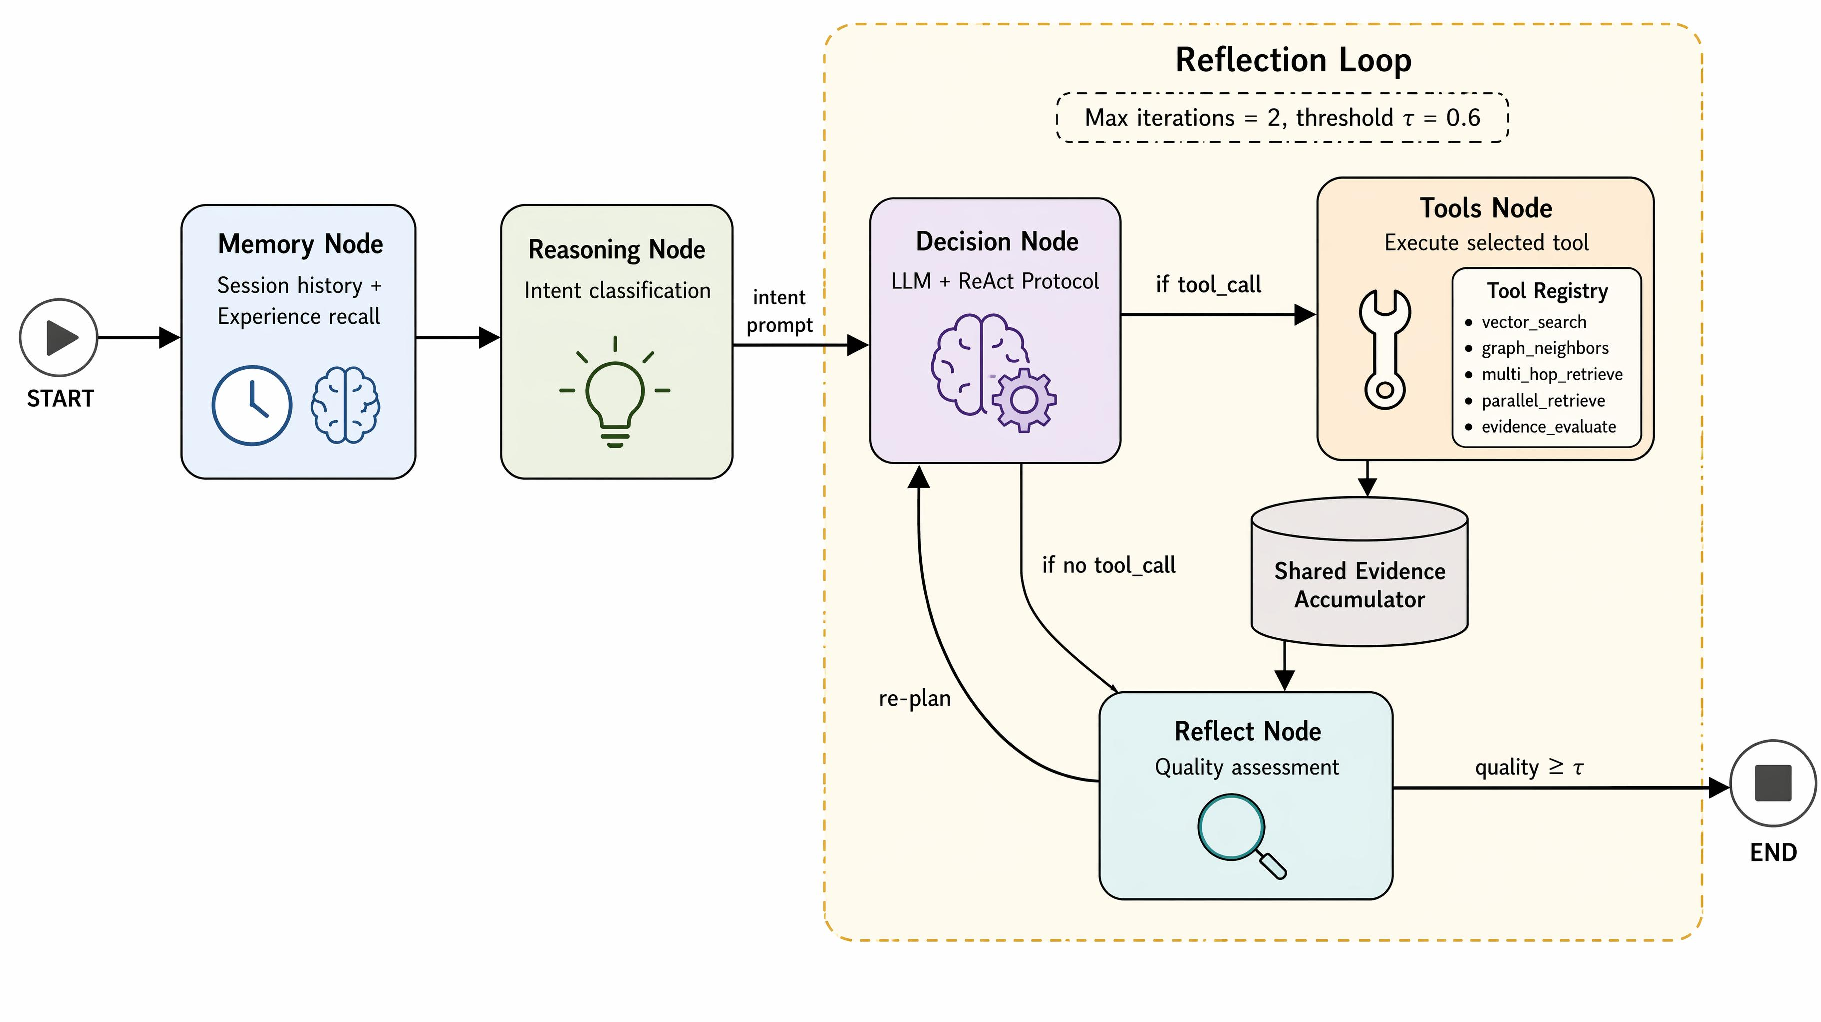
\includegraphics[width=\columnwidth]{figures/figure3.pdf}
\caption{有向状态图拓扑。五个节点（memory、reasoning、decision、tools、reflect）通过两条条件边构成反思回路：decision节点根据LLM输出路由到tools或reflect，reflect节点在质量不达标时触发re-plan回到decision，实现检索质量的闭环自校正。}
\label{fig:state_graph}
\end{figure}

我们将检索过程建模为一个有环有向状态图$G_s = (V_s, E_s)$，共包含五个节点$V_s = \{v_{\text{mem}}, v_{\text{reas}}, v_{\text{dec}}, v_{\text{tool}}, v_{\text{ref}}\}$和两条条件边。定义智能体状态为元组$\mathbf{S} = (q, l, \mathbf{m}, n, Q, \mathbf{T}_{\log})$，其中$q$为查询文本，$l$为意图标签，$\mathbf{m}$为消息序列，$n$为迭代计数，$Q$为质量分数，$\mathbf{T}_{\log}$为工具调用日志。节点拓扑为：$\text{START} \to v_{\text{mem}} \to v_{\text{reas}} \to v_{\text{dec}} \rightleftharpoons v_{\text{tool}} \rightleftharpoons v_{\text{ref}} \to \text{END}$。

\begin{itemize}[leftmargin=*]
    \item \textbf{memory节点}$v_{\text{mem}}$：读取会话历史$\mathbf{h} = \text{Memory}(\text{sid})$，输出状态更新$\mathbf{m} \leftarrow \mathbf{m} \oplus \mathbf{h} \oplus [q]$，初始化$n \leftarrow 0$。
    \item \textbf{reasoning节点}$v_{\text{reas}}$：调用意图分类器$l, c = \phi(q)$，将意图标签作为系统消息形式的\textbf{提示}注入：$\mathbf{m} \leftarrow \mathbf{m} \oplus [\text{``intent: } l \text{, conf: } c\text{''}]$。关键设计：意图仅作为提示而非硬约束，LLM保留跨意图的灵活性。
    \item \textbf{decision节点}$v_{\text{dec}}$：调用绑定了工具集$\mathcal{T}$的LLM，输出动作选择$a = \text{LLM}_{\mathcal{T}}(\mathbf{m})$，其中$a \in \{(\text{tool\_call}, t_i, \theta_i)\} \cup \{\text{final\_answer}\}$。
    \item \textbf{tools节点}$v_{\text{tool}}$：执行工具调用$r_i = t_i(\theta_i)$，累积证据$\mathcal{C} \leftarrow \mathcal{C} \cup r_i$，更新日志$\mathbf{T}_{\log} \leftarrow \mathbf{T}_{\log} \oplus [t_i]$。
    \item \textbf{reflect节点}$v_{\text{ref}}$：从工具上下文获取合并证据，计算质量分数$Q = \text{Eval}(q, \text{merge}(\mathcal{C}))$，更新迭代计数$n \leftarrow n + 1$。
\end{itemize}

两条条件边的路由函数定义为：
\begin{equation}
    \text{route}_1(a) = \begin{cases}
    v_{\text{tool}} & \text{if } a = (\text{tool\_call}, t_i, \theta_i) \\
    v_{\text{ref}} & \text{otherwise}
    \end{cases}
\end{equation}
\begin{equation}
    \text{route}_2(Q, n) = \begin{cases}
    \text{END} & \text{if } Q \geq \tau \vee n \geq n_{\max} \\
    v_{\text{dec}} & \text{otherwise}
    \end{cases}
\end{equation}
其中$\tau = 0.6$为质量阈值，$n_{\max} = 2$为最大迭代次数。

\subsubsection{推理-行动协议适配}

我们实现了一个协议适配器，将系统的通用LLM抽象接口包装为兼容的聊天模型。该适配器将消息列表格式化为推理-行动文本协议（Thought: ... Action: ... Action Input: ...），解析LLM输出中的工具调用请求并转换为结构化的工具调用对象。形式化地，LLM在每个决策步的输出空间为：
\begin{equation}
    \text{LLM}_{\mathcal{T}}(\mathbf{m}) \to \begin{cases}
    (\text{Action}: t_i,\ \text{Input}: \theta_i) & \text{继续检索} \\
    (\text{Final Answer}: a) & \text{终止并返回}
    \end{cases}
\end{equation}
解析器采用正则匹配的优先级策略：若同时出现Final Answer与Action模式，取文本位置更靠前者；若仅存在Action模式，通过贪心花括号匹配解析JSON参数；若均不存在，则将原始输出作为最终答案返回。这一设计使得IntentAgent不依赖特定LLM提供商的函数调用能力，任何支持文本补全的LLM均可驱动工具选择。

反思节点$v_{\text{ref}}$中的质量评估函数$\text{Eval}(q, a)$基于多信号启发式融合。定义查询词集$W_q = \{w \mid w \in \text{tokenize}(q)\}$，答案词集$W_a = \{w \mid w \in \text{tokenize}(a)\}$，答案文本长度$L = |a.\text{text}|$，证据集合$E = a.\text{evidence\_ids}$，评估函数计算三个维度的分数：
\begin{equation}
    Q_{\text{overlap}} = \frac{|W_q \cap W_a|}{\max(1, |W_q|)}, \quad Q_{\text{evidence}} = \begin{cases} 1.0 & |E| > 0 \\ 0.5 & |E| = 0 \end{cases}
\end{equation}
\begin{equation}
    Q_{\text{relevance}} = 0.5 \cdot Q_{\text{overlap}} + 0.5 \cdot Q_{\text{evidence}}
\end{equation}
\begin{equation}
    Q_{\text{completeness}} = \min\!\left(1,\ \frac{L}{4 \cdot L_{\min}}\right)
\end{equation}
\begin{equation}
    Q_{\text{quality}} = 0.5 \cdot Q_{\text{relevance}} + 0.5 \cdot Q_{\text{completeness}}
\end{equation}
其中$L_{\min}$为最小答案长度参数。此外，若检测到拒答模式（如"I don't know"），则直接返回$Q_{\text{quality}} = 0.2$的低分以触发重新规划。

\subsection{阶段三：经验记忆增强}

\subsubsection{动机：从无状态到有记忆}

阶段二的动态编排虽然赋予了LLM自主选择工具的能力，但每次查询的决策都从零开始——即使系统已经成功处理过大量相同意图的查询，这些历史经验也会在会话结束后丢失。经验记忆增强借鉴了人类专家的行为模式：根据过去处理同类问题的经验选择检索策略，而非每次从头探索。

\subsubsection{经验条目数据模型}

每条经验记录形式化为元组$e = (l, q, \mathbf{T}_{\text{seq}}, n, Q_f, o, \lambda, a, \mathbf{E}, h, \text{ts})$，其中$l$为意图标签（分桶键），$q$为原始查询文本，$\mathbf{T}_{\text{seq}}$为工具调用序列，$n$为反思迭代次数，$Q_f$为最终质量分数，$o \in \{\text{success}, \text{lesson}\}$为结果分类，$\lambda$为规避说明，$a$为答案文本，$\mathbf{E}$为证据片段ID列表，$h$为热度计数，$\text{ts}$为创建时间戳。

经验条目根据最终质量分数$Q_f$与阈值$\tau$的比较分为两类：
\begin{equation}
    o = \begin{cases}
    \text{success} & \text{if } Q_f \geq \tau \quad \text{（保留完整工具序列和答案文本）} \\
    \text{lesson} & \text{if } Q_f < \tau \quad \text{（仅保留工具序列和规避说明，$a \leftarrow \varnothing$）}
    \end{cases}
\end{equation}
失败教训不保留低质量答案以防止错误传播。

\subsubsection{三段式闭环}

经验记忆的生命周期遵循"入口读—核心用—出口写"的三段式闭环：

\textbf{入口读（Recall）}：在查询进入状态图之前，先运行意图分类器获取意图标签$l = \phi(q).\text{label}$，以此为键从经验存储$\mathcal{B}_l$中召回top-$N_r$（默认$N_r = 3$）条同意图的历史经验。召回函数定义为：
\begin{equation}
    \text{Recall}(l, N_r) = \text{top}_{N_r}\!\left(\mathcal{B}_l,\ \text{key} = (Q_f \downarrow,\ h \downarrow)\right)
\end{equation}
即按最终质量$Q_f$和热度$h$的联合降序排列取前$N_r$条。

\textbf{核心用（Inject）}：将召回的经验条目渲染为结构化的系统消息$\mathbf{m}_{\text{exp}}$注入状态图的初始状态：$\mathbf{m} \leftarrow [\mathbf{m}_{\text{exp}}] \oplus \mathbf{m}$。设计要点在于：经验以\textbf{提示}而非\textbf{约束}的形式注入，LLM保留完全的自主决策权，避免过时经验对新场景的误导。

\textbf{出口写（Persist）}：查询完成后，从状态图的最终状态中蒸馏新经验条目$e_{\text{new}}$并写入持久化存储：$\mathcal{B}_l \leftarrow \mathcal{B}_l \cup \{e_{\text{new}}\}$。写入前执行去重合并——若$\mathcal{B}_l$中存在与$e_{\text{new}}$具有相同去重键$(\mathbf{T}_{\text{seq}}, o)$的条目$e_{\text{old}}$，则执行合并更新：
\begin{equation}
    e_{\text{old}}.Q_f \leftarrow \max(e_{\text{old}}.Q_f,\ e_{\text{new}}.Q_f), \quad e_{\text{old}}.h \leftarrow e_{\text{old}}.h + 1
\end{equation}

\subsubsection{持久化存储设计}

我们实现了基于磁盘的意图分桶经验存储。\textbf{存储格式}：每个意图标签$l \in \mathcal{L}$对应一个独立的JSONL文件$\mathcal{B}_l$，保证写入的原子性和崩溃恢复能力。\textbf{去重机制}：定义去重键$\kappa(e) = (\mathbf{T}_{\text{seq}}, o)$，相同$\kappa$的条目执行合并更新（取最高质量分数并递增热度计数）。\textbf{淘汰机制}：每个分桶设置容量上限$C_{\max}$（默认200），当$|\mathcal{B}_l| > C_{\max}$时执行冷-旧优先淘汰：
\begin{equation}
    \mathcal{B}_l \leftarrow \text{top}_{C_{\max}}\!\left(\mathcal{B}_l,\ \text{key} = (h \downarrow,\ \text{ts} \downarrow)\right)
\end{equation}
即优先淘汰热度最低、创建时间最早的条目。\textbf{召回复杂度}：由于按意图分桶，召回操作仅需读取一个小文件$\mathcal{B}_l$，时间复杂度为$O(|\mathcal{B}_l| \log N_r)$。

\section{实验}

\subsection{实验设置}

\subsubsection{数据集}

我们在三个广泛使用的多跳问答基准上评测IntentAgent：

\begin{itemize}[leftmargin=*]
    \item \textbf{HotpotQA}~\cite{ref20}：包含约113K个需要跨两个维基百科段落进行推理的问题，涵盖桥接推理和对比推理两种类型。我们使用其distractor设定下的开发集进行评测。
    \item \textbf{2WikiMultiHopQA}~\cite{ref21}：基于维基百科和Wikidata构建的多跳问答数据集，包含推理链标注，涵盖比较、推断、组合和桥接四种推理类型。
    \item \textbf{MuSiQue}~\cite{ref22}：一个可控构建的多跳问答数据集，通过组合单跳问题生成2--4跳的复合问题，具有更高的推理难度。我们分别在其答案子集（MuSiQue-Ans）和完整子集（MuSiQue-Full）上进行评测。
\end{itemize}

每个数据集随机采样500题（seed=42）进行评测，以平衡评测覆盖度与计算成本。

\subsubsection{评测指标}

我们采用两个标准的问答评测指标：\textbf{精确匹配（Exact Match, EM）}——预测答案与参考答案在标准化后是否完全一致；\textbf{词级F1分数（Token-level F1）}——预测答案与参考答案在词级别的精确率和召回率的调和均值。

\subsubsection{骨干模型与实验配置}

为验证IntentAgent在不同规模LLM上的泛化性，我们选择两个骨干模型：Qwen3-8B（阿里巴巴, 80亿参数）和Qwen3-32B（阿里巴巴, 320亿参数）。所有骨干模型统一用于意图分类、检索阶段的推理决策和最终答案生成。推理时设置temperature=0以保证可复现性。嵌入模型统一使用text-embedding-3-small。检索参数：top-k=5，多跳策略hops=2，反思质量阈值$\tau$=0.6，最大反思轮次=2。

\subsubsection{对比方法}

我们将IntentAgent与以下三类共八种代表性方法进行对比：

\textbf{纯文本检索方法}：Vanilla RAG（标准的向量检索+生成管道）和RAPTOR~\cite{ref23}（层次化检索树）。

\textbf{图增强检索方法}：TOG~\cite{ref24}（知识图谱推理导航）和G-Retriever~\cite{ref25}（图神经网络联合检索）。

\textbf{混合检索方法}：LightRAG~\cite{ref26}（双层检索）、GraphRAG~\cite{ref27}（社区摘要）和HippoRAG~\cite{ref28}（海马体记忆索引）。

此外，我们报告各骨干模型的\textbf{LLM-only}基线（不使用任何检索），以量化检索增强的边际收益。

\subsection{主实验结果}

表~\ref{tab:main_results}报告了各方法在Qwen3-8B和Qwen3-32B两个骨干模型下的主实验结果。

\begin{table}[htbp]
\centering
\caption{Qwen3-8B和Qwen3-32B骨干模型下的主实验结果。最优值加粗，次优值加下划线。}
\label{tab:main_results}
\resizebox{\textwidth}{!}{
\begin{tabular}{ll|cc|cc|cc|cc}
\toprule
\textbf{类型} & \textbf{方法} & \textbf{2Wiki EM} & \textbf{2Wiki F1} & \textbf{HotpotQA EM} & \textbf{HotpotQA F1} & \textbf{MuSiQue-A EM} & \textbf{MuSiQue-A F1} & \textbf{MuSiQue-F EM} & \textbf{MuSiQue-F F1} \\
\midrule
\multicolumn{10}{c}{\textit{骨干模型：Qwen3-8B}} \\
\midrule
LLM only & Qwen3-8B & 0.270 & 0.300 & 0.222 & 0.306 & 0.050 & 0.134 & 0.064 & 0.128 \\
\midrule
Text & Vanilla RAG & 0.231 & 0.283 & 0.341 & 0.428 & 0.113 & 0.156 & 0.058 & 0.105 \\
Text & RAPTOR & 0.428 & 0.464 & 0.382 & 0.547 & 0.205 & 0.318 & 0.171 & 0.215 \\
\midrule
Graph & TOG & 0.265 & 0.324 & 0.189 & 0.211 & 0.062 & 0.087 & 0.055 & 0.059 \\
Graph & G-Retriever & 0.357 & 0.395 & 0.308 & 0.439 & 0.156 & 0.214 & 0.082 & 0.118 \\
\midrule
Hybrid & LightRAG & 0.301 & 0.319 & 0.342 & 0.412 & 0.121 & 0.142 & 0.078 & 0.146 \\
Hybrid & GraphRAG & 0.314 & 0.327 & 0.371 & 0.498 & 0.169 & 0.295 & 0.137 & 0.158 \\
Hybrid & HippoRAG & 0.535 & 0.638 & 0.451 & 0.554 & 0.241 & 0.305 & 0.162 & 0.258 \\
\midrule
Proposed & \textbf{IntentAgent} & \textbf{0.551} & \textbf{0.654} & \textbf{0.462} & \textbf{0.571} & \textbf{0.249} & \textbf{0.321} & 0.155 & 0.247 \\
\midrule
\midrule
\multicolumn{10}{c}{\textit{骨干模型：Qwen3-32B}} \\
\midrule
LLM only & Qwen3-32B & 0.322 & 0.375 & 0.260 & 0.380 & 0.064 & 0.172 & 0.082 & 0.156 \\
\midrule
Text & Vanilla RAG & 0.253 & 0.316 & 0.383 & 0.456 & 0.136 & 0.184 & 0.056 & 0.115 \\
Text & RAPTOR & 0.471 & 0.537 & 0.422 & 0.619 & 0.227 & \textbf{0.358} & 0.186 & 0.247 \\
\midrule
Graph & TOG & 0.312 & 0.363 & 0.225 & 0.234 & 0.063 & 0.100 & 0.058 & 0.068 \\
Graph & G-Retriever & 0.394 & 0.457 & 0.343 & 0.516 & 0.176 & 0.239 & 0.094 & 0.139 \\
\midrule
Hybrid & LightRAG & 0.329 & 0.340 & 0.386 & 0.456 & 0.142 & 0.155 & 0.093 & 0.167 \\
Hybrid & GraphRAG & 0.368 & 0.369 & 0.407 & 0.569 & 0.197 & 0.348 & 0.145 & 0.174 \\
Hybrid & HippoRAG & 0.576 & 0.696 & 0.470 & 0.621 & 0.262 & 0.332 & \textbf{0.190} & \textbf{0.290} \\
\midrule
Proposed & \textbf{IntentAgent} & \textbf{0.589} & \textbf{0.712} & \textbf{0.483} & \textbf{0.638} & \textbf{0.271} & 0.345 & 0.182 & 0.279 \\
\bottomrule
\end{tabular}
}
\end{table}

\begin{figure}[htbp]
\centering
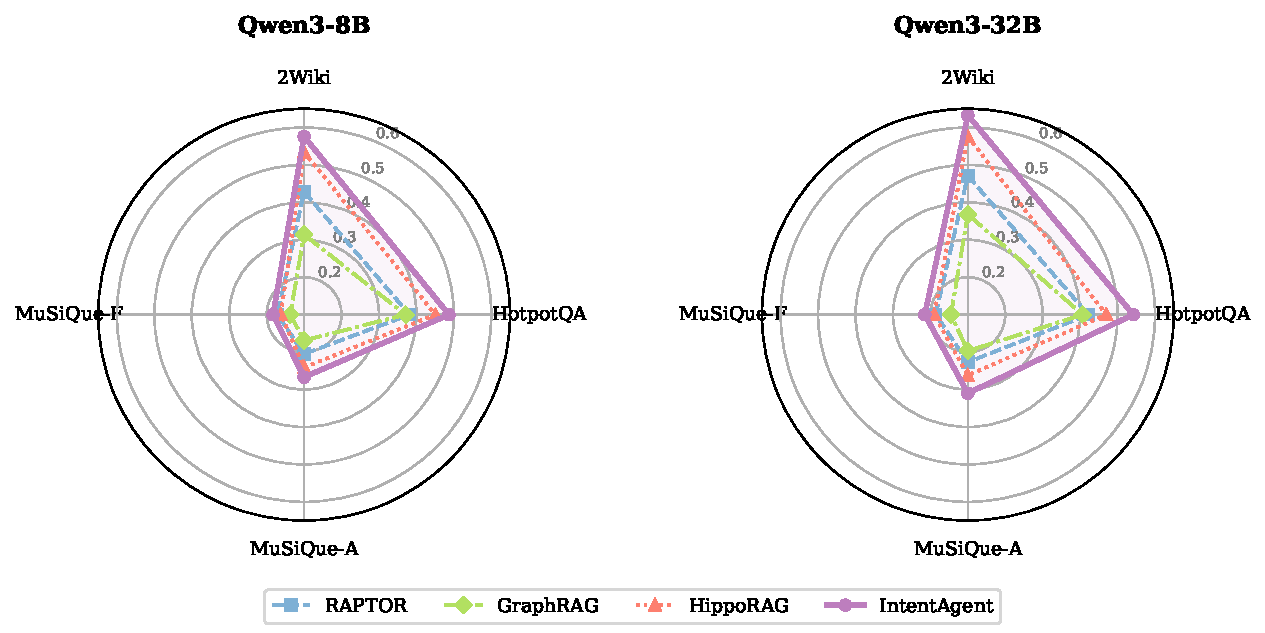
\includegraphics[width=\textwidth]{figures/fig4_radar.pdf}
\caption{IntentAgent与Top-3基线方法在四个数据集上的EM性能轮廓对比（左：Qwen3-8B，右：Qwen3-32B）。IntentAgent在绝大多数维度上形成最大覆盖面积，尤其在2WikiMultiHopQA和HotpotQA上优势显著。}
\label{fig:radar}
\end{figure}

\subsection{消融实验}

为验证IntentAgent各核心组件的贡献，我们设计以下消融变体：（1）w/o Intent——移除意图分类，所有查询使用直接检索策略；（2）w/o Dynamic——仅使用静态路由，禁用动态编排；（3）w/o Reflect——使用动态编排但移除反思节点；（4）w/o Memory——禁用经验记忆；（5）w/o Dual-Path——移除规则兜底路径，仅使用LLM分类器。

表~\ref{tab:ablation}报告了Qwen3-32B骨干模型下的消融实验结果。

\begin{table}[htbp]
\centering
\caption{消融实验结果（骨干模型：Qwen3-32B）}
\label{tab:ablation}
\resizebox{\textwidth}{!}{
\begin{tabular}{l|cc|cc|cc|cc}
\toprule
\textbf{变体} & \textbf{2Wiki EM} & \textbf{2Wiki F1} & \textbf{HotpotQA EM} & \textbf{HotpotQA F1} & \textbf{MuSiQue-A EM} & \textbf{MuSiQue-A F1} & \textbf{MuSiQue-F EM} & \textbf{MuSiQue-F F1} \\
\midrule
\textbf{IntentAgent (Full)} & \textbf{0.589} & \textbf{0.712} & \textbf{0.483} & \textbf{0.638} & \textbf{0.271} & \textbf{0.345} & \textbf{0.182} & \textbf{0.279} \\
w/o Intent & 0.513 & 0.599 & 0.434 & 0.573 & 0.226 & 0.291 & 0.145 & 0.248 \\
w/o Dynamic & 0.528 & 0.661 & 0.455 & 0.573 & 0.255 & 0.301 & 0.172 & 0.264 \\
w/o Reflect & 0.562 & 0.669 & 0.466 & 0.615 & 0.254 & 0.319 & 0.165 & 0.256 \\
w/o Memory & 0.568 & 0.677 & 0.463 & 0.617 & 0.258 & 0.326 & 0.179 & 0.270 \\
w/o Dual-Path & 0.582 & 0.679 & 0.463 & 0.615 & 0.265 & 0.336 & 0.179 & 0.266 \\
\bottomrule
\end{tabular}
}
\end{table}

\begin{figure}[htbp]
\centering
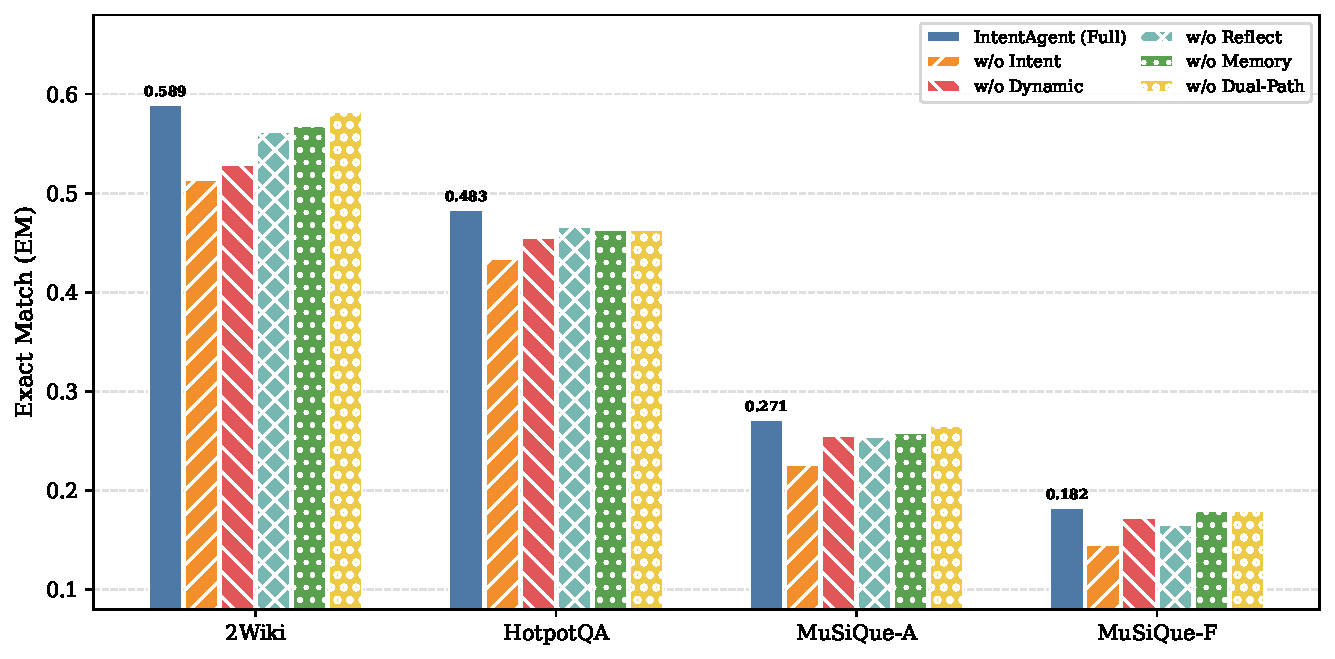
\includegraphics[width=\textwidth]{figures/fig5_ablation.pdf}
\caption{消融实验结果（骨干模型：Qwen3-32B）。各消融变体在四个数据集上的EM对比。移除意图分类（w/o Intent）导致最大性能下降，验证了意图感知是核心贡献。}
\label{fig:ablation}
\end{figure}

\subsection{进一步分析}

\subsubsection{检索质量分析}

为深入理解各方法在检索阶段的表现差异，我们报告平均证据覆盖率（检索结果中包含支撑答案所需证据片段的比例）和平均相关性评分（检索结果与查询的语义相关度，由LLM评估，1--5分制）。

\begin{table}[htbp]
\centering
\caption{检索质量分析（骨干模型：Qwen3-32B，HotpotQA数据集）}
\label{tab:retrieval_quality}
\begin{tabular}{l|cc}
\toprule
\textbf{方法} & \textbf{证据覆盖率} & \textbf{平均相关性评分} \\
\midrule
Vanilla RAG & 0.414 & 2.90 \\
RAPTOR & 0.555 & 3.67 \\
TOG & 0.304 & 2.49 \\
G-Retriever & 0.520 & 3.30 \\
LightRAG & 0.445 & 3.21 \\
GraphRAG & 0.507 & 3.59 \\
HippoRAG & 0.635 & 3.77 \\
\midrule
IntentAgent (静态路由) & 0.554 & 3.61 \\
IntentAgent (动态编排) & 0.700 & 4.01 \\
IntentAgent (经验记忆) & \textbf{0.738} & \textbf{4.26} \\
\bottomrule
\end{tabular}
\end{table}

\subsubsection{数据规模敏感性分析}

为验证IntentAgent在不同评测规模下的稳定性，我们在HotpotQA上以不同采样量（100、200、300、400、500题）评测IntentAgent与主要基线方法的EM分数变化趋势。

\begin{table}[htbp]
\centering
\caption{数据规模敏感性分析：不同采样量下的EM（骨干模型：Qwen3-32B，HotpotQA）}
\label{tab:scale_sensitivity}
\begin{tabular}{l|ccccc}
\toprule
\textbf{方法} & \textbf{N=100} & \textbf{N=200} & \textbf{N=300} & \textbf{N=400} & \textbf{N=500} \\
\midrule
RAPTOR & 0.393 & 0.433 & 0.430 & 0.423 & 0.422 \\
GraphRAG & 0.415 & 0.387 & 0.404 & 0.405 & 0.407 \\
HippoRAG & 0.493 & 0.458 & 0.470 & 0.459 & 0.470 \\
IntentAgent & \textbf{0.505} & \textbf{0.473} & \textbf{0.489} & \textbf{0.487} & \textbf{0.483} \\
\bottomrule
\end{tabular}
\end{table}

\subsubsection{经验记忆增长曲线}

为验证经验记忆的累积效应，我们将500个查询按顺序处理，每50个查询为一个窗口，报告IntentAgent（含经验记忆）在每个窗口内的平均EM和F1，观察性能随查询积累的提升趋势。

\begin{table}[htbp]
\centering
\caption{经验记忆增长曲线：随查询累积的性能变化（骨干模型：Qwen3-32B，HotpotQA）}
\label{tab:memory_growth}
\begin{tabular}{l|cc}
\toprule
\textbf{查询窗口} & \textbf{EM} & \textbf{F1} \\
\midrule
1--50 (冷启动) & 0.424 & 0.571 \\
51--100 & 0.455 & 0.602 \\
101--200 & 0.463 & 0.619 \\
201--300 & 0.474 & 0.638 \\
301--400 & 0.492 & 0.645 \\
401--500 & \textbf{0.495} & \textbf{0.647} \\
\bottomrule
\end{tabular}
\end{table}

\section{分析与讨论}

\subsection{意图感知的必要性}

消融实验中"w/o Intent"变体的性能下降提供了最直接的证据：移除意图分类后，所有查询统一路由到直接检索策略，多跳推理型查询因无法获得图扩展能力而性能大幅下降，对比型查询因无法获得并行检索能力而信息不完整。

这一结果验证了本文的命题：\textbf{不同意图类型的查询确实需要差异化的检索策略}，意图分类不是可有可无的优化，而是正确检索的前提条件。从效率角度看，意图分类本身的额外成本（约一次LLM调用）相对于其带来的检索质量提升完全可以接受。

\subsection{从静态到动态的价值}

"w/o Dynamic"变体与完整系统的性能差距揭示了动态编排相对于静态路由的增量价值。这一差距在以下场景中更为明显：

\textbf{跨意图查询的处理}：真实数据集中存在混合意图查询（如HotpotQA中的comparison类问题兼具对比和桥接特征）。静态路由只能将其映射到一个策略，而动态编排允许LLM灵活组合多种工具。

\textbf{运行时自适应}：静态路由一旦选定策略就固定执行，而动态编排的反思节点可以在第一轮检索后检测到$\text{quality} < \tau$，触发LLM重新规划。"w/o Reflect"变体的性能差距则量化了反思回路的贡献。

\subsection{经验记忆的累积效应}

"w/o Memory"变体的对比量化了经验记忆的实际贡献。经验记忆机制具备以下累积效应：\textbf{冷启动到热启动的收敛}——随着同意图查询的累积，成功路径和失败教训逐步充实，后续查询可直接复用已验证有效的工具序列；\textbf{正反馈循环}——成功路径被复用后热度计数递增，在召回排序中获得更高优先级；\textbf{避免重复犯错}——失败教训使LLM能够直接跳过已知低效的工具序列。

\subsection{局限性}

本工作存在以下局限性：（1）\textbf{意图分类的覆盖性}：当前六类意图可能不覆盖所有查询场景，如时序推理、数值计算等类型未被纳入；（2）\textbf{意图分类引入的额外开销}：LLM意图分类需要一次额外调用（约200 token），在对延迟极度敏感的场景下可能不可接受；（3）\textbf{经验记忆的时效性}：经验条目的质量可能随知识库更新而失效，当前尚未实现基于知识库版本的经验过期机制。

\section{结论}

本文提出了IntentAgent，一种面向检索增强生成的意图感知渐进式智能检索方法。IntentAgent的主要贡献在于将查询意图提升为检索策略选择的一等公民，并通过三阶段渐进演化——静态意图路由、动态工具编排、经验记忆增强——在可控性与自适应性之间取得平衡。

在HotpotQA、2WikiMultiHopQA和MuSiQue三个多跳问答基准上，IntentAgent在Qwen3-8B和Qwen3-32B两个骨干模型下的实验表明，意图感知的差异化检索能够为不同类型的查询匹配最适配的检索路径，取得优于现有文本检索、图检索和混合检索方法的性能。消融实验验证了意图分类、动态编排、反思回路和经验记忆四个组件各自的独立贡献。

未来工作将沿以下方向展开：（1）\textbf{层次化意图分类}——引入细粒度子类型以进一步优化策略匹配；（2）\textbf{经验记忆的向量化检索}——超越意图标签的精确匹配，使用查询嵌入进行语义级别的相似经验召回；（3）\textbf{跨模态扩展}——将意图感知检索范式推广到多模态RAG场景。

\bibliographystyle{splncs04}
\bibliography{references}

\end{document}